
\providecommand{\myrootdir}{..}
\documentclass[\myrootdir/main.tex]{subfiles}

\begin{document}

\chapter{Information Retrieval Techniques}
\label{sec:models}
%\includegraphics[page=1, width=\textwidth, trim={0.5cm 0.5cm 0.5cm 0.5cm}, clip]{img/RetreatSeptemberSlides.pdf}
Many different information retrieval techniques ... this section describes the conceptional / theoretical results of our thesis ...
We create a model to characterize BLIE techniques so we can discuss their similarities and differences more clearly.
Additionally we present a complimentary model for IE tasks, to describe use cases for BLIE techniques in a structured way.
From our analysis of build logs we share our notion of the retrievable information within a build log.

\section{Characteristics of a Build Log}
The idea of CI is, to integrate new software changes fast and often to catch errors early~\cite{humble2010continuous}.
After making a change, the developer commits and pushes it to a shared source code repository. Companies often use a specific CI server, e.g. Travis CI, linked to their source code repository.
A CI build might then be triggered by a push on specific branches or after a pull request was created.
When such a CI build is triggered, it typically runs through these stages:

\begin{itemize}
	\item \todo{look for more in modelling paper zampetti}
	\item Pulling the new, changed version of the source code onto the server.
	\item Running static analysis tools~\cite{zampetti2017open}.
	\item Building the software, i.e. compiling and packaging it~\cite{phillips2014understanding}.
	\item Running automated tests~\cite{beller2017oops}.
\end{itemize}

However these are only \emph{typical} stages and there is a high variability in the CI build processes of different software projects \mention{citation needed, zampetti2017open?}.
Some smaller projects might use CI to just make sure their code compiles as a minimal check before reviewing a pull request.
Other projects might have various stages of extensive automated testing.

Most software tools used within a build will write out log messages to the console \mention{citation needed, paper about usages of console.log?}.
To communicate progress updates, error and warning messages to the user.
This combined output is referred to as build log.
The structure of their output is chosen by every tool themselves.
Many have implicit or explicit structuring rules, some adhere to predefined standards \mention{phpunit, ruby, xuint output?}.
\todo{figure X} shows how different tools contribute to the whole build log.

When analyzing build logs we might not have access to the exact build configuration, describing which tools are used in which order, or might not have access to a useable definition of the output structure of a specific tool.
As the structure of a build log is not known to us, we describe build logs as semi-structured. Section \ref{sec:rw-semi-structured-data} describes different properties of semi-structured data.

\section{Retrievable Information in Build Logs}
\begin{figure}[h]
  \centering
\includegraphics[page=2, width=\textwidth, trim={0.5cm 0.5cm 0.5cm 0.5cm}, clip]{img/flow-of-research.pdf}
  \caption{Information retrievable from build logs}
  \label{fig:build-log-information-draft}
\end{figure}
Continuous integration build logs contain a huge amount of information about the various stages in the CI build they correspond to.
In this section we present a model, which more precisely describes our notion of a information retrievable from a CI build log.

The central class of our model is the \emph{build log information} (BLI), representing an piece of information possibly retrievable from a build log.
\emph{Possibly}, because a build log information is not necessarily present in every build log.
If it is present, we call it a \emph{build log information instantiation} (BLII), which always relates to a specific build log, the one it is appearing in.
\todo{add to model, build, build log, bulidloginformationinstantiation as association name to the type build log information}
Each BLII for us has a \emph{textual representation} within the build log.
This textual representation is always a substring of the log text.
With this build log information \todo{akward class names like BuildLogInformation? s would be possible then} can be hierarchically ordered by their textual representations containing each other.
As this is an ad-hoc and a-posteriori structuring schema, as we describe in Section \ref{sec:rw-semi-structured-data}, the model only presents hierarchical ordering or containment for build log informations whose structure we definetely know.
Most build log information types can appear in various hierarchical arrangements and therefore not contained in any other type in the model.

\begin{figure}[h]
	\centering
	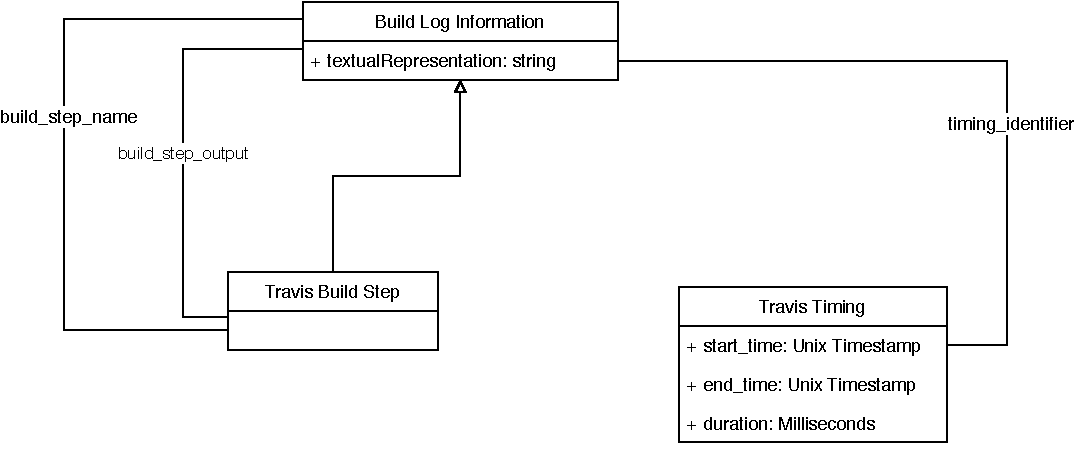
\includegraphics[width=\textwidth]{img/mt-graphics-BuildLogInformation.pdf}
	\caption{Build Log Information}
	\label{fig:build-log-information}
\end{figure}
During our initial exploration and log data collection for the \emph{Failing Build Log Data Set}, we collected a broad set of build logs from 29 languages and 87 repositories. We inspected them to get an impression about the information one would want to retrieve from a build log. Within the build logs from Travis CI we found various different information types possibly interesting to be retrieved:

\begin{itemize}
	\item \textbf{Travis Build Step} A Travis CI build consists of several build steps defined within the Travis CI configuration language. Within the build log each of these steps are framed by \lstinline{travis_fold:start:<build step name>} and \\ \lstinline{travis_fold:end:<build step name>}.
	These build steps could be categorized, for example into \textbf{Test Step}, \textbf{Linter Step}, \textbf{Travis Worker}, \textbf{Git Fetch}, or \textbf{Sudoers} are some that we encountered in the logs.
	A build step contains
	\begin{itemize}
		\item \textbf{Build Step Name} The string Travis CI uses to identify the step within start and end statements.
		\item \textbf{Build Step Output} The output generated during the build step. The textual representation of the \texttt{Build Step Output} Instantiation is the substring between the start and end statements.
	\end{itemize}
	You can see an example of a Travis Build Step and its components within a build log in Figure \ref{fig:log-1}.

	\item \textbf{Non-Travis Build Step??}
	\item 
	\item \textbf{Travis Timing} Travis can measure the time of specified sections of the build process.
	You can see an example of a Travis Build Step and its components within a build log in Figure \ref{fig:log-1}.
	%It represents those by \lstinline{travis_time:start:<timing section id>} and \\ \lstinline{travis_time:end:<timing section id>:start=<start time>,finish=<finish time>,duration=<duration>}

	\item \textbf{Travis Worker} Travis CI mentions for each build which machine is executing it.
	Retrieving this information from multiple build logs could for example help visualize the impact of the build server assignment algorithm.
	The Travis Worker is a good example to show that the same BLI can have different textual representations in different build logs.
	You can see examples of Travis Worker instantiations in Figure \ref{fig:log-0} and Figure \ref{fig:log-2}.

	\item \textbf{Travis System Info} At the beginning of each log Travis CI describes the tech stack of the server executing the build.
	The system info could be retrieved from both failing and successful logs and compared to identify if a failure is possibly based on the execution environment.
	You can see an example of a Travis System Info instantiation within a build log in Figure \ref{fig:log-0}.

	\item \textbf{Triggering Command} Travis CI logs the commands it uses to call certain tools.
	These come from the \texttt{travis.yml} configuring the build.
	Retrieving this information from the log could for example be useful when reverse engineering the build configuration.
	You can see an example of a Triggering Command instantiation within a build log in Figure \ref{fig:log-3}.

	\item \textbf{Exit Code} Travis CI prints all exit codes of commands.
	This information could be used to fill an overview of the build steps and why they failed.
	You can see an example of an Exit Code instantiation within a build log in Figure \ref{fig:log-3}.

	\item \textbf{Error Message} Various tools involved in the build process might output messages of errors that occurred during their execution.
	Retrieving these and showing them to developers could help them understand quicker why the build failed.
	You can see an example of and Error Message instantiation within a build log in Figure \ref{fig:log-3}.

	\item \textbf{Warning Message} In addition to errors, tools also print warning messages.
	These could be collected, counted and presented to developers, encouraging them to resolve them in order to improve their software.
	You can see examples of WarningMessage instantiations within build logs in Figure \ref{fig:log-4} and Figure \ref{fig:log-5}.

	\item \todo{name, explanation, ref to example image, example what to be used for}
\end{itemize}

\begin{figure}[h]
	\centering
	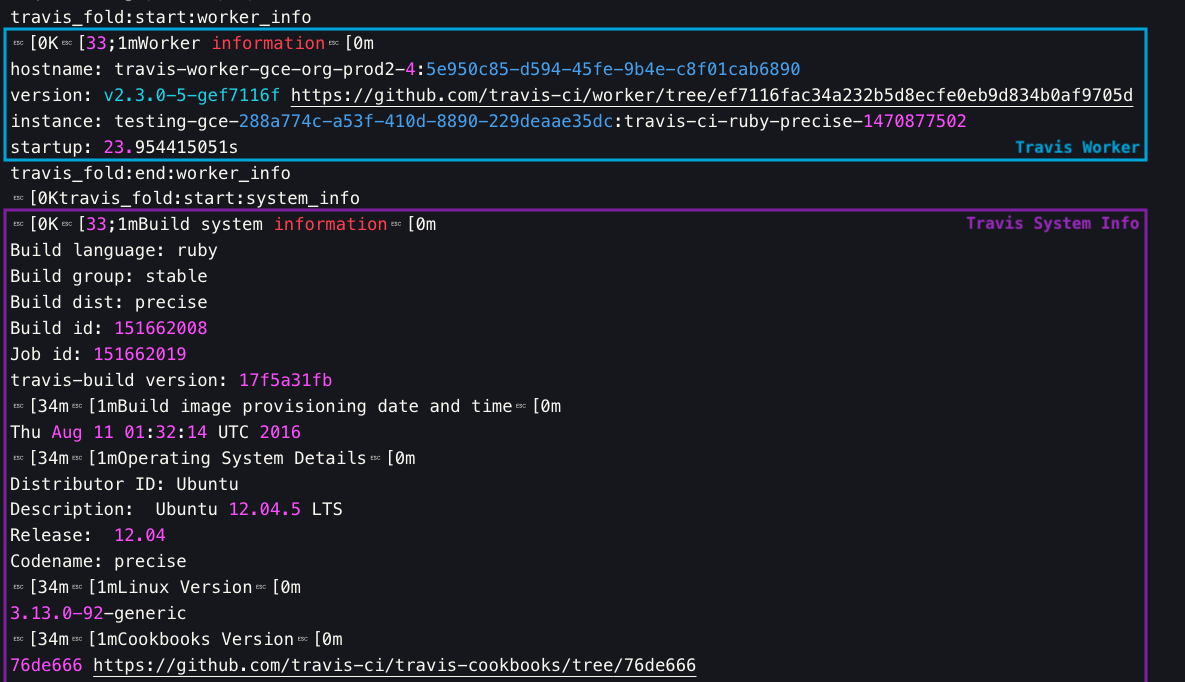
\includegraphics[width=\textwidth, clip]{img/log0.png}
	\caption{Excerpt from a build log showing textual representations of a long Travis Worker instantiation and a Travis System Info instantiation}
	\label{fig:log-0}
\end{figure}
\begin{figure}[h]
	\centering
	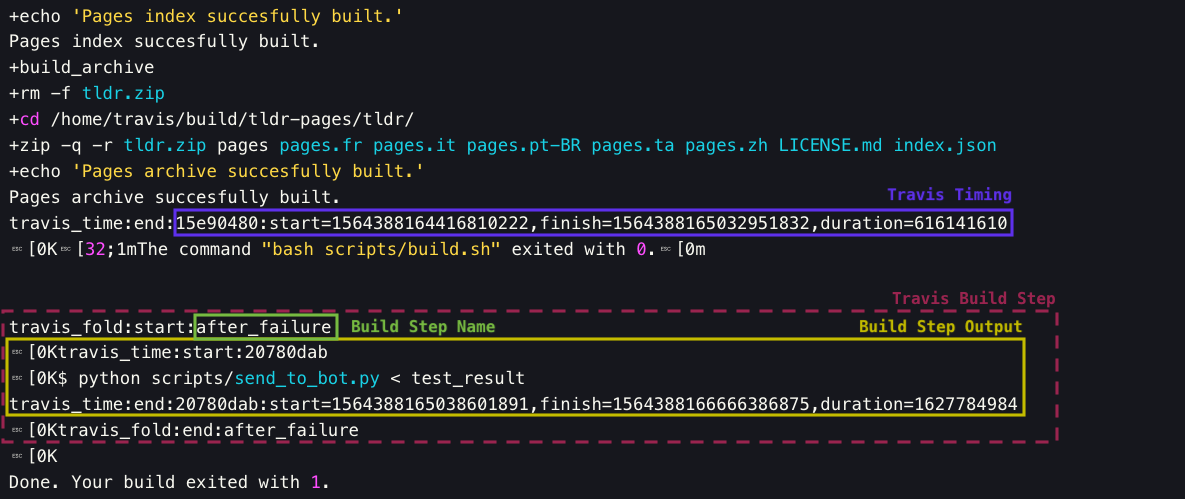
\includegraphics[width=\textwidth, clip]{img/log1.png}
	\caption{Excerpt from a build log showing textual representations of a Travis Timing instantiation and a Travis Build Step, containing the Build Step Name and the Build Step Output}
	\label{fig:log-1}
\end{figure}
\begin{figure}[h]
	\centering
	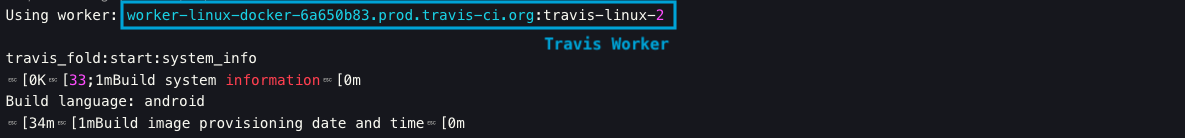
\includegraphics[width=\textwidth, clip]{img/log2.png}
	\caption{Excerpt from a build log showing textual representations of a short Travis Worker instantiation}
	\label{fig:log-2}
\end{figure}
\begin{figure}[h]
	\centering
	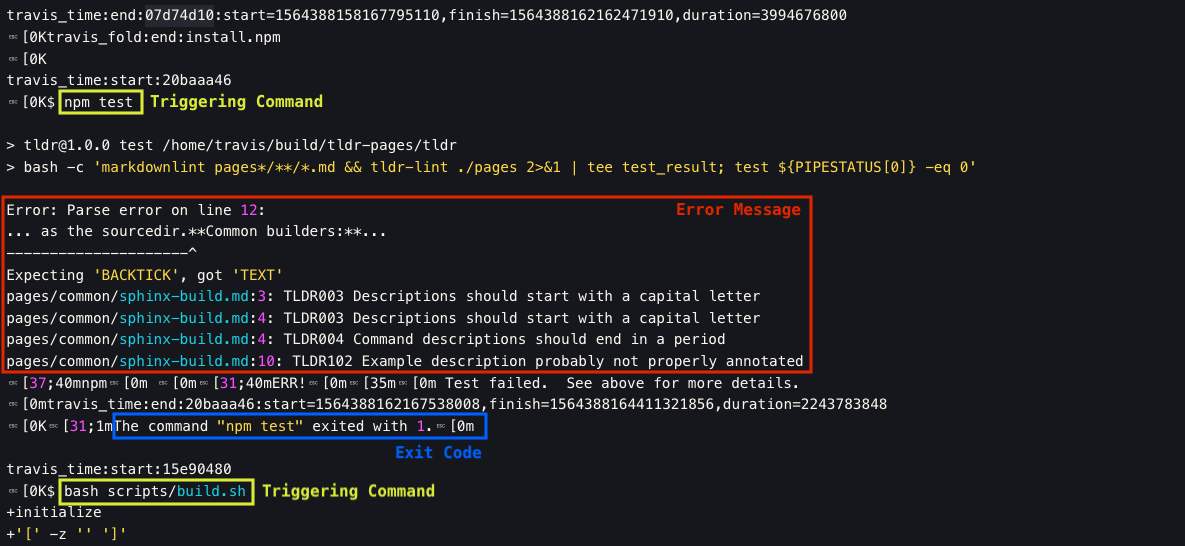
\includegraphics[width=\textwidth, clip]{img/log3.png}
	\caption{Excerpt from a build log showing textual representations of Error Message, Exit Code and Triggering Command instantiations}
	\label{fig:log-3}
\end{figure}
\begin{figure}[h]
	\centering
	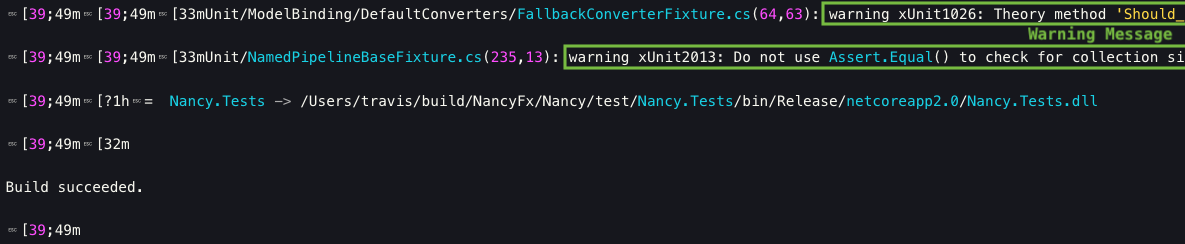
\includegraphics[width=\textwidth, clip]{img/log4.png}
	\caption{Excerpt from a build log showing textual representations of Warning Message instantiations}
	\label{fig:log-4}
\end{figure}
\begin{figure}[h]
	\centering
	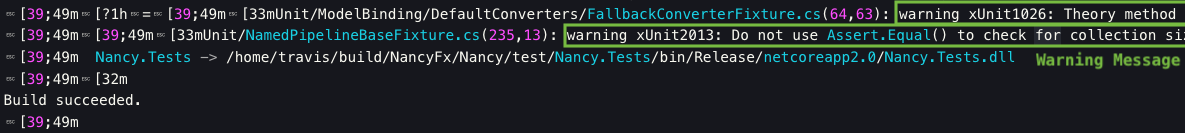
\includegraphics[width=\textwidth, clip]{img/log5.png}
	\caption{Excerpt from a build log showing textual representations of Warning Message instantiations}
	\label{fig:log-5}
\end{figure}


\section{Characteristics of Information Retrieval Techniques}
\begin{figure}[h]
	\centering
	\includegraphics[page=3, width=\textwidth, trim={0.5cm 0.5cm 0.5cm 0.5cm}, clip]{img/flow-of-research.pdf}
	\caption{Model for an information retrieval technique}
	\label{fig:model-ie-technique}
\end{figure}
For this thesis we want to evaluate different information retrieval techniques in their application to CI build logs. We focus on techniques that do not attempt or require to parse the structure of a whole build log, but rather focus on extracting just one specific information
A build log information retrieval technique (BLIR technique) consumes a build log (text file) and produces a certain output (text). \todo{make picture, output can be contained in log or not, can be continuous substring or selected lines etc.}.
\begin{itemize}
	\item \textbf{Target}{Extractable Information} each retrieval technique \todo{instantiation!} targets a specific information
	\item \textbf{Setup Overhead} {Time}
	\item \textbf{Performance} {Performance} split into learning performance
	\item \textbf{Configuration Scope} for one repository/project, a language/logkind, global
	\item \textbf{Granularity} of extraction, i.e. the smallest extractable text piece
\end{itemize}

Example instantiations of this task later in this chapter, namely for the three techniques we are comparing: PROSE program synthesis, IR text similarity, and simple keyword search. \todo{ref?}

\section{Information Retrieval Tasks}
\begin{figure}[h]
	\centering
	\includegraphics[page=4, width=\textwidth, trim={0.5cm 0.5cm 0.5cm 0.5cm}, clip]{img/flow-of-research.pdf}
	\caption{Model for information extraction task}
	\label{fig:modelt-ie-task}
\end{figure}
aims to describe an information retrieval task of a developer or a researcher.
\begin{itemize}
	\item \todo{describe all classes}
	\item{Setup Overhead}{Time}
	\item{Performance}{Performance} split into learning performance
	\item 
\end{itemize}
\todo{give 2-3 concrete example instantiations here}


\section{PROSE Program Synthesis}
\begin{figure}[h]
  \centering
\includegraphics[page=2, width=\textwidth, trim={0.5cm 0.5cm 0.5cm 0.5cm}, clip]{img/RetreatSeptemberSlides.pdf}
  \caption{Synthesizing regular expression programs by example using PROSE}
  \label{fig:prose-explanation}
\end{figure}
\subsection*{Overview}
\emph{Programming by Example (PBE)} is a technique where programs are synthesized according to in and output examples provided by the user. It enables users to create programs without requiring programming knowledge~\cite{mayer2015user}. Applied A to the task of text extraction through regular expressions it relieves the developer from having to understand the whole document structure to solve a single extraction task~\cite{le2014flashextract:}.
We chose to investigate the applicability of generating regular expression programs by example to extracting information from build logs. In this work we refer to our interpretation of this technique as \emph{PBE}. \todo{distinguish PBE for buildlogs}

Generally, we are interested in whether a Programming by Example could replace manually writing regular expressions.
Writing and especially maintaining regular expressions is known to be a difficult, tedious and error-prone task~\cite{michael2019regexes}.
There are two ways to approach this question: from the usability side or the technical side.

When studying the applicability of PBE from the \emph{usability} perspective you run into questions like
\begin{itemize}
	\item Are users faster when using PBE compared to manual regex construction?
	\item Are users more comfortable using PBE over manual regex construction?
	\item Are users confident in the resulting regular expression program from PBE?
	\item Are the resulting extractions more or less accurate when using PBE over manual regex construction?
\end{itemize}
Some of these were already evaluated in existing works about PBE and user interaction~\cite{mayer2015user} \mention{other works?}.
Adequately answering those questions is however highly dependent on the user interface and the corresponding interaction model used during a study.
Developers who are accustomed to crunching on regular expressions in their favorite IDE or Editor might have an adversely negative view on syntesizing programs from examples in an unknow interface.
Mayer et al.~\cite{mayer2015user} presented two system-user interaction models to improve the confidence of users into the programs synthesized from their examples.
We feel such questions of usability can be answered separately from the application domain of build logs.

For our work we chose to look at the applicability of PBE from the \emph{technical} perspective.
We investigate whether current program synthesis techniques are able to learn programs for information retrieval tasks in the domain of CI build logs.
Furthermore we gather insights in how PBE has to be applied to yield useable results and perform best.
Our implementation of PBE \todo{which we name technique name x}, is mainly based on the Flash Extract DSL~\cite{flahsextractpaper} of the PROSE library by Microsoft\mention{cite prose website}.
Due to that our technique of text extraction through regular expression programs synthesized is highly influenced by the capabilities of Flash Extract.
In the following we will explain the concept of how we apply PBE to information retrieval from CI build logs, the concrete implementation is described in \ref{sec:impl-pbe}.

\subsection*{Configuration / Input / Output}
In/Output examples (I/O examples) are the main driver of Programming by Example.
When extracting information from build logs the \emph{input} is always a whole build log, i.e. the whole text of the build log file without any preprocessing.
In the implementation we did have to apply a few text replacements as described in \ref{sec:impl-preprocessing}.
The \emph{output} is always a substring of the log file text, representing the substring that should be extracted by the syntesized program when given the corresponding input file.
One or multiple I/O examples are needed as configuration for PBEBL, they are used to define substring of a log should be extracted.
For execution PBEBL takes a build file as input and returns a substring of the build file content.

\subsection*{Synthesizing Programs with Flash Extract}
\todo{maybe scrap this section / incorporate last sentence somewhere else, expalnation will mostly be in rw. How to usefully sturcture the stuff above this?}
In the following we want to give an impression on how the PROSE library and specifically the Flash Extract DSL synthesize programs for extracting substrings from text via regular expressions.
\todo{how much can/should we explain here? possibly big parts are already explained in related work: vsa, divied and coquer, witness functions, enumeration and ranking (prose theory paper), flash extract specifics like what functions they have (absolute pos, pre/post regex), rankings specific to ci biulg logs?}
Our approach is based on the Flash Extract DSL, which in turn is based on the FlashMeta algorithm. Both are described in \todo{ref rw sections}.

\subsection*{Model instantiation}


\section{Text Similarity}
\begin{figure}[h]
  \centering
\includegraphics[page=3, width=\textwidth, trim={0.5cm 0.5cm 0.5cm 0.5cm}, clip]{img/RetreatSeptemberSlides.pdf}
  \caption{Extracting information using text similarity}
  \label{fig:text-similarity-explanation}
\end{figure}
\paragraph{Overview}
Text Similarity approaches are more and more used to filter unstructured textual software artifacts. \mention{cite papers that do exactily this. also lda possbible here}
One common and simple technique the Vector Space Model \mention{citation needed, for VSM and that it is common maybe?}.
We investigate when it is a suitable technique to retrieve information from build logs.

\paragraph{Configuration / Input / Output}
To configure a retrieval though text similarity we chose to use the same concept of I/O examples as for PBE.
The output strings of a given example set define our search query.
A retrieval run then takes as input a log file and outputs the parts most similar to the search query.

\paragraph{Similariy Calculation}
The TS retrieval technique works on a granularity of lines.
First, the search query is processed.
The output strings of the example set configuring the technique are split into single lines.
For each line we apply preprocessing: Splitting it into tokens, in our case words.
%Commonly text similarity techniques employ further normalization like removing special characters and stop words.
%We chose to keep the build log lines as complete as possible, as we often saw special characters and words identifying an interesting area.
Then we build a document-term-frequency matrix over the lines of the output strings and prune very often or very rarely appearing words.
Next, the algorithm applies term-frequency inverse document frequency, a best practice for natural language queries~\cite{lee1997document}.
To retrieve the desired information from a build log, we parse the whole text and process it in the same way.
The algorithm calculates the cosine simlarity~\mention{citation?} to compare each line of the build log with each line of the search query.
After summing up the similarities of each build log line to all the query lines, we sort the build log lines in decreasing similarity.
The average number of lines in the I/O example output strings determines how many of the most similar lines are returned as the output of the retrieval run.

\paragraph{Instantiate Retrieval Technique Model}


%Information retrieval techniques are more and more prevalently used to extract textual information from unstructured textual sources~\mention{stuff annibale is referencing?}. We describe CI build logs as semi-structured, 

\section{Keyword Search}
\begin{figure}[h]
  \centering
\includegraphics[page=4, width=\textwidth, trim={0.5cm 0.5cm 0.5cm 0.5cm}, clip]{img/RetreatSeptemberSlides.pdf}
  \caption{Extracting information using keyword search}
  \label{fig:keword-search-explanation}
\end{figure}

\paragraph{Overview}
When we are looking for a specific information within a great amount of unstructured information, a first ad-hoc approach is to search for keywords in the text we assume to be near the information we are looking for.
This was one of the most common approaches we took when searching for the build failure reason within a log when creating our data set.
As this is a technique readily available in many tools developers use to view build logs, we want to study when such a simple search for keywords is recommendable for retrieving information from CI build logs.

\paragraph{Configuration / Input / Output}
SKWS is configured by giving a set of keywords.
For a retrieval run we then take a whole build log file as input and search for all exact occurrences of the keywords.
As keywords are often not directly describing the desired information but rather adjacent to the desired information, this technique not only retrieves the line with the keyword, but only the context around it.
We chose a context of 10 lines above and below the keyword appearance.

\paragraph{Instantiation of Model}

\todo{explanation of process, the way our tool does it, instantiate model of retrieval technique, probably no additional theoretical stuff really needed here?}

\section{Further Techniques}
\todo{maybe: instantiate model, or at least partly talk about it}
\todo{diffing, manual regex?, other summarization?, BART? <- we could reference that from related work then}

\end{document}
